\chapter{Asking Millionaires How To Make \$1{,}000{,}000!}

This chapter follows a School of Hard Knocks interview, curated by LazyingArt LLC. We are not given a blackboard lecture, but a moving sequence of doorstep questions in wealthy Austin neighborhoods. The notes therefore do something slightly unusual: we keep the rhythm of the search, the refusals, the resets, and the strongest interviews, while extracting from them a compact set of mechanisms about work, saving, ownership, market fit, patience, reputation, and optionality.

\begin{remark}
No validated board figures survive for this chapter. The equations below are therefore not transcriptions of visible mathematics; they are compact reconstructions of the business logic spoken in the interview.
\end{remark}

\section{Method: Asking in Public, Learning Under Rejection}

The lecture begins not with a theory of wealth but with a method for getting one. We are taken through one of the wealthiest neighborhoods in Texas, and the host states the project plainly: go door to door, ask millionaires how they became wealthy, and keep going until the answers become transferable. The first refusal is therefore important. It is not a detour; it establishes the cost of the inquiry.

Later the host makes this explicit by saying that the success rate is easily below five percent. In other words, the lecture treats rejection not as atmosphere, but as data about the difficulty of extracting useful information from the world:
\begin{equation}
p_{\text{successful interview}} < 0.05.
\end{equation}
That inequality is not the point by itself. The point is that the inquiry is iterative. We ask, are refused, adjust, and ask again. Before any advice about business appears, the episode already models one of its own lessons: persistence has to precede insight.

\section{Career Entry: Difficulty, Initiative, and Best Practices}

The first substantial interview comes from a man who pursued natural gas. His advice is severe and memorable: choose the most difficult, most challenging, most dangerous job you can find, work harder than anybody else, and if you see a problem, do not wait for someone else to fix it. The lecture begins here because it wants a first rule with sharp edges. Wealth, in this framing, begins with a willingness to move toward difficulty rather than away from it.

\paragraph{Claim.}
Hard work is not presented as moral decoration. It is tied to problem ownership. The interviewee's principle is not merely to labor more, but to notice what is wrong, trace the cause, and solve it.

\paragraph{Mechanism.}
In a compressed, editorial form, the first path in the lecture may be written as
\begin{align}
\text{difficulty} &\longrightarrow \text{initiative} \longrightarrow \text{responsibility}, \\
\text{problem noticed} &\longrightarrow \text{cause identified} \longrightarrow \text{value created}.
\end{align}
When the host asks about the most money made in a single year, the answer is framed as cash flow of roughly half a million dollars:
\begin{equation}
C_{\text{cash flow}} \approx \$5\times 10^{5}\ \text{yr}^{-1}.
\end{equation}
The numerical point is modest but useful. The interview is not selling fantasy scale; it is linking a career ethic to an operating income figure.

The next interview complicates the picture. A president of a software company in industrial IoT says that his first job was at a startup and that he learned a great deal, but if he had to do it again he might first work at a large company in order to absorb best practices before returning to a smaller one. That is a genuine counterpoint. The lecture does not collapse into one slogan. We are given a second path:
\begin{align}
\text{large firm} \longrightarrow \text{best practices} \longrightarrow \text{smaller-firm leverage}.
\end{align}
The host also preserves another concrete rule from this exchange: begin in a city with many options, so that mobility across firms remains possible. Already we can see the chapter's early tension. One answer prizes raw difficulty and initiative; the next insists on sequence, apprenticeship, and institutional learning.

\section{Ownership Versus Employment}

After more refusals, the host stops to narrate the rejection rate and then resets for day two. This reset matters. The lecture is teaching us how to continue under discouraging odds just before it arrives at its strongest conceptual answer.

A former professional basketball player, now involved in a sports ownership group with teams around the world, is asked for his best advice to someone starting a business. His answer becomes the central spine of the episode: do not spend your life only building for someone else. If we are going to give our time to something, we should try, when we can, to grow something that is truly ours.

\begin{definition}
We shall call \emph{optionality} the size of the set of career and business moves one can realistically choose without immediate financial distress.
\end{definition}

The interview immediately adds the necessary qualification. Ownership is desirable, but it is difficult when we are young. Therefore the rule is not ``quit immediately.'' The rule is: work, save money for a few years, and then use that saved runway to build something one can own.

\begin{figure}[h]
\centering
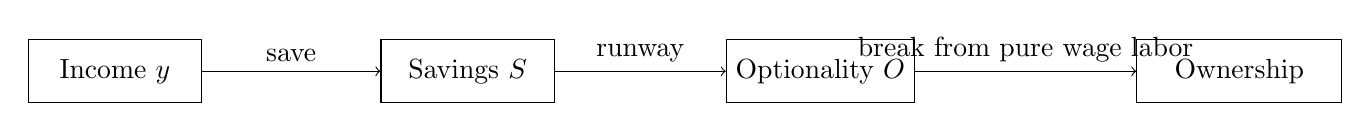
\begin{tikzpicture}[x=2.8cm,y=1.1cm]
\node[draw, rectangle, minimum width=2.2cm, minimum height=0.8cm] (income) at (0,0) {Income \(y\)};
\node[draw, rectangle, minimum width=2.2cm, minimum height=0.8cm] (savings) at (1.6,0) {Savings \(S\)};
\node[draw, rectangle, minimum width=2.2cm, minimum height=0.8cm] (option) at (3.2,0) {Optionality \(O\)};
\node[draw, rectangle, minimum width=2.6cm, minimum height=0.8cm] (own) at (5.1,0) {Ownership};

\draw[->] (income) -- node[above] {save} (savings);
\draw[->] (savings) -- node[above] {runway} (option);
\draw[->] (option) -- node[above] {break from pure wage labor} (own);
\end{tikzpicture}
\caption{Editorial reconstruction of the lecture's main mechanism: earn, save, widen the set of feasible moves, and then attempt ownership.}
\end{figure}

\subsection{Question \& Answer}

\paragraph{Question.}
If ownership is superior to employment, why does the lecture not simply tell us to leave salaried work at once?

\paragraph{Answer.}
Because the obstacle is not desire but feasibility. The interview insists that young people usually cannot jump directly into ownership without first building savings and endurance. The bridge from employment to ownership is not rhetoric. It is runway.

If \(S(t)\) denotes saved resources, \(y\) labor income, \(s\) the savings rate, and \(c\) the rate of consumption, the spoken mechanism can be summarized by the update rule
\begin{equation}
S(t+\Delta t)=S(t)+s\,y\,\Delta t-c\,\Delta t.
\end{equation}
The same point can be written even more directly as
\begin{equation}
O=O(S), \qquad \frac{dO}{dS}>0.
\end{equation}
More savings mean more runway, and more runway means more options. That is the lecture's closing language in embryo.

A simple worked version makes the logic concrete. Let
\begin{equation}
\sigma = s\,y-c
\end{equation}
be annual surplus after saving and spending. If one needs a threshold \(S^\star\) of savings before leaving employment to build something owned, then in discrete yearly steps we have
\begin{align}
S_{n+1} &= S_n + \sigma, \\
S_n &= S_0 + n\sigma.
\end{align}
Therefore the first year \(n\) at which the leap becomes feasible satisfies
\begin{equation}
n \ge \frac{S^\star-S_0}{\sigma}.
\end{equation}
This is the lecture's practical answer to its own question. Ownership is not opposed to patience; it depends on it.

To keep the larger structure clear, we may summarize the wealth path schematically by
\begin{equation}
W \approx W_{\text{labor}} + W_{\text{ownership}}.
\end{equation}
The interview plainly privileges the second term over the long run, but it also shows how the first term finances entry into the second.

\section{Scale, Teams, and the Reading of Character}

The next major interview shifts from the ownership principle to the architecture of a large enterprise. We hear of a broadcasting business that grew to roughly 350 radio stations, of a first station bought at age twenty-nine, and of a year in which the sale of the company produced on the order of fifty million dollars:
\begin{equation}
X_{\text{company sale}} \approx \$5\times 10^{7}.
\end{equation}
Here the lecture does something interesting with scale. It first shows us spectacle, then rapidly refuses to let spectacle be the lesson. The interviewee says that starting a business is really about the people one is connected to, learning to communicate, building a great team, trusting them, having a good business plan, and then going for it.

\paragraph{Anecdote.}
The large exit is the memorable number.

\paragraph{Claim.}
The durable mechanism is team construction and communication.

\paragraph{Mechanism.}
The interview then sharpens the point with a criterion for selecting people: look for someone who has had some failure. The lecture's reasoning is that we see more of a person's business character after the fall and recovery than in a spotless upward line. In compact form,
\begin{equation}
\text{failure} + \text{recovery} \Longrightarrow \text{evidence about character}.
\end{equation}
This is not a theorem. It is a hiring heuristic. But it is one of the lecture's clearest attempts to turn story into selection rule.

\section{Market Homework and Local Fit}

After another host aside about how strange the whole process can appear to homeowners, the lecture pivots from inner qualities to market realism. A trial lawyer, who also once owned part of three bars in Houston, gives the chapter its best local business diagnostic: do your homework.

The example is specific. A new pizza place opens in Westlake. At first this sounds promising. Then the interviewee discovers that it sells slices. His objection is not culinary; it is structural. Slices make sense where foot traffic is high, as in Times Square. They do not automatically make sense in a lower-foot-traffic pocket near a supermarket in Westlake.

This is the closest the lecture comes to an explicit commercial model. Let \(D\) denote local demographics, \(F\) local foot traffic, and \(P\) product format. Then the lecture's point is
\begin{equation}
D_{\text{local demographics}} \text{ and } F_{\text{foot traffic}} \text{ must fit } P_{\text{product format}}.
\end{equation}
We may package that relation as a market-fit function,
\begin{equation}
M = M(D,F,P).
\end{equation}
What the anecdote shows is that a business can fail without any deep mystery if \(M\) is weak. In particular, the lecture suggests that the product ``pizza by the slice'' is not portable across locations. The relevant question is not simply whether the product is good, but whether the product format is matched to the tempo and density of local demand.

\paragraph{Mechanism.}
The diagnostic sequence is simple:
\begin{enumerate}
\item Identify the business format \(P\).
\item Ask what sort of passing customer flow \(F\) it requires.
\item Ask whether the surrounding population \(D\) will supply that flow.
\item If not, the business may be ill-fitted before management quality even enters.
\end{enumerate}
The lecture is careful here. It does not claim omniscience. It asks a better question: who did their homework?

\section{Skill, Capital, and Investment Horizon}

The next cluster of interviews broadens the field while keeping the rhythm of concrete rules. One interviewee says he was CEO and founder of two technical companies, one acquired by Intel and one, MyVest, acquired by TIAA. His advice is stripped down almost to a minimum: learn a lot, get a marketable skill, and master it. This is a useful counterweight to the glamour of exits. Before capital multiplies, competence has to exist.

From there the lecture moves into investment timing. The answer given is telling: timing is difficult, so do not make timing the core of the rule. Instead, insist that the capital committed be money one will not need for perhaps ten years:
\begin{equation}
T_{\text{investment horizon}} \approx 10\ \text{years}.
\end{equation}
That shift is pedagogically important. The lecture does not promise that we can forecast the market. It substitutes a horizon condition for a prediction condition.

When the host asks about the most money made in a single year, the answer is intentionally imprecise: seven digits, but not more specific. The most honest way to preserve that claim is interval-valued:
\begin{equation}
Y_{\max} \in [10^{6},10^{7}) \text{ dollars}.
\end{equation}

The shorter interviews continue to stack transferable rules. A professor with a background in software engineering says that long-term real-estate investing was a good financial decision. The humorous aside about marrying a successful lawyer should remain as color, but not as mechanism. The mechanism is the long-term holding logic, not the joke.

\section{Persistence, Conviction, and Optionality}

The final run of the lecture sounds at first like a mosaic of short interviews, but it resolves into one connected argument. First we hear from a sales career: what separates people is persistence, the willingness to keep going, and the willingness to reevaluate when something is not working. The lecture is subtle here. Persistence is not stubborn repetition. It is endurance with adjustment.

Then we hear from a real-estate developer in Austin. The advice is to know what one is going after, know the market, make fast decisions, and have conviction about them. That is strong advice, but it is immediately constrained by a second instruction: keep a good name, maintain a good reputation, and treat investors properly.

If \(R_t\) denotes reputation capital at time \(t\), the closing discipline may be summarized by
\begin{equation}
R_{t+1}=R_t+\Delta R_{\text{good conduct}}-\Delta R_{\text{bad conduct}}.
\end{equation}
The point of writing the rule is not to quantify reputation precisely. It is to show that the lecture refuses to separate speed from trust. Fast action without reputation is not treated as mastery.

The same interview opens into the final answer of the chapter. There is opportunity in many layers of real estate: cutting lawns, buying and selling properties, buying land, development. The trick is not to worship a single slot in the industry, but to find the slot one understands and then act quickly, cleanly, and consistently.

The host's last big question asks how someone can start becoming wealthy now. The reply returns us to the savings problem. When the brokerage career began, it began with a partner and with enough savings to make the commitment. Without those savings, the interviewee says, the choice would not have existed. This is the lecture's closing theorem in ordinary language: without financial stability, one loses optionality.

We may write the final thought in the deliberately schematic form
\begin{equation}
\frac{dO}{dS}>0,
\end{equation}
where \(O\) is optionality and \(S\) is savings. The lecture's conclusion is not that savings are glamorous. It is that savings enlarge the feasible set of lives one can actually choose.

\section{Summary}

The lecture begins with doors, not formulas, but its structure is tight. First we learn that the search for useful advice itself requires persistence under rejection. Then we are given competing but compatible rules for career entry: move toward difficult work, and learn best practices where they exist. The central answer follows on day two: if possible, do not spend your whole life building only for someone else; save first, then try to own what you are building. From there the lecture descends into mechanism: teams matter, recovered failure reveals character, business models must fit local markets, investing requires horizon, sales require persistence, real estate requires conviction joined to reputation, and savings preserve optionality.

That last word is the right one to end on. The chapter does not offer a secret technique for instant wealth. It offers a sequence of constraints and practices by which the space of possible futures becomes wider rather than narrower.